\chapter{Results: What Was Good and Where Were the Compromises}
\label{chapter:results}

\section{Targeting Different Platforms}
\label{section:targeting-platforms}

Despite the web browser being the unified environment for different
platforms, there are lots of differences between various devices. The
form factors vary from tiny mobile screens to touch screen tablets and
desktop monitors and each device and platform has its own feature
set. There are also known bugs in the browsers that have to be
handled.

Therefore, means to detect the user's device are needed. Here we
present two such means: device detection and feature detection. Both
of these were used in our conference application.

\subsection{Device Detection}
\label{subsection:device-detection}

The User-Agent (\abbr{UA}) \abbr{HTTP} header contains detailed
information of the web browser and platform where the request
originates. As we can see from Table~\ref{table:user-agents}
(\fixme{Check table ref number}), we can extract platform and browser
specific information from the UA header.

\begin{table}
  \begin{tabular}{ l | l | p{7cm} }
    \textbf{Device} & \textbf{Platform} & \textbf{User-Agent} \\ \hline
    Samsung Nexus S & Android 2.3.4 & Mozilla/5.0 (Linux; U; Android 2.3.4; en-us; Nexus S Build/GRJ22) AppleWebKit/533.1 (KHTML, like Gecko) Version/4.0 Mobile Safari/533.1 \\ \hline
    Apple iPhone & iOS 3.1.3 & Mozilla/5.0 (iPhone; U; CPU iPhone OS 3\_1\_3 like Mac OS X; de-de) AppleWebKit/528.18 (KHTML, like Gecko) Version/4.0 Mobile/7E18 Safari/528.16 \\ \hline
    Apple iPad & iOS 5.0 & Mozilla/5.0 (iPad; CPU OS 5\_0 like Mac OS X) AppleWebKit/534.46 (KHTML, like Gecko) Mobile/9A334 \\ \hline
    Unknown & Android & Opera/9.80 (Android; Opera Mini/6.5.26571/26.1023; U; de) Presto/2.8.119 Version/10.54 \\ \hline
  \end{tabular}
  \label{table:user-agents}
  \caption{Example User-Agent strings.}
\end{table}

In the conference application, device detection was used in the
backend to provide a different offline AppCache manifest to different
device groups. The detection was also used in defining the assets to
be preloaded in the application. The devices were divided into four
categories based on the rules defined in
Table~\ref{table:device-detection-rules} (\fixme{Check table ref
  number}). There were serious limitations in this approach, and
compromises had to be made.

First, there is no way to surely know if the device actually is what
it reports itself to be. Second, the most important thing to know when
generating the screen specific assets in the manifest file would have
been the screen size. However, this information is not present in the
UA header. We could have listed all the assets for all the devices,
but then the list of offline assets would have grown too much and, for
example, have large images also for older mobile phones.

Despite the drawbacks, the received advantages of this approach
outweighed the possible compromises. The worst that could happen was
that the device was wrongly classified and the proper resources were
not downloaded for offline use.

\begin{table}
  \begin{tabular}{ l | l }
    \textbf{Rule} & \textbf{Device Type} \\ \hline
    'iPad' in UA & highres \\
    'iPhone' in UA & iphone \\
    'Android 3' in UA & highres \\
    'mobile' (case insensitive) in UA & mobile \\
    'MIDP' in UA & mobile \\
    'Opera Mobi' in UA & mobile \\
    'Opera Mini' in UA & mobile \\
    otherwise (desktop computer) & highres
  \end{tabular}
  \label{table:device-detection-rules}
  \caption{Device type detection rules.}
\end{table}

Getting platform and browser information from the UA header might look
tempting and useful, but it is considered a bad practice to detect a
device from it and provide device specific bug fixes or additional
features. The header can easily be changed and some browsers or
browser plugins even provide preconfigured values for certain browsers
or devices for spoofing. Also, the device specific bug fixes might
become obsolete with platform updates, and the application might break
due to invalid expectations. This is why feature detection is
generally the recommended option whenever possible.

\subsection{Feature Detection}

Feature detection is an important concept in Progressive Enhancement
design (See Section~\ref{subsection:progressive-enhancement}). A lot
of the HTML5 related JavaScript APIs are still unsupported in several
platforms, but browser developers are constantly filling the
gaps. Therefore, it is important to check whether a certain feature is
supported and provide graceful fallback mechanisms for browsers
lacking the functionality.

Doing runtime feature detection provides the possibility to give
additional functionality to modern browsers and instant support for
devices that add the feature support in the lifetime of the
application. In the conference application (\fixme{ref needed?}), we
used the Modernizr feature detection library (\fixme{already ref
  earlier, add bib entry?}) to check for HTML5 features.

For example, the user could add sessions to his or her favorites by
clicking the star in the agenda or on the session details view
(\fixme{add screenshot?}). The favorites were then listed on the home
view together with information about the time left for them to begin.

We used HTML5 localStorage for storing the favorites in the user's web
browser. By using Modernizr, we detected localStorage support and
showed the favorite stars only in browsers that supported the
functionality. For all other browsers, the stars were simply hidden
and users could not add favorites. We could have also provided a
fallback mechanism for persisting the favorites to the backend, but
for simplicity and because we targeted mostly modern platforms, this
approach was considered as reasonable.

\section{Targeting Different Screens}
\label{section:targeting-screens}

Probably the biggest difference in various devices and form factors is
the screen size, resolution, and dimensions. Web applications should
adjust to the available space and flexible handle screen orientation
and window size changes.

First, to target mobile and tablet platforms, the viewport meta
information should be indicated in the document. The following tag was
used in the conference application:

\begin{verbatim}
<meta name="viewport" content="width=device-width,
                               initial-scale=1.0">
\end{verbatim}

The viewport meta tag was first introduced in Apple's iPhone and
afterwards ported to other platforms, such as Android. The possible
configuration options and default values might vary between
platforms. Values accepted by Android are shown in
Table~\ref{table:viewport-meta} (\fixme{Check table ref number})
\citationneeded. iOS devices also support these same properties.

\begin{table}
  \begin{tabular}{ l | l | p{5cm} }
    \textbf{Property} & \textbf{Description} & \textbf{Value} \\ \hline
    height & Height of the viewport. & pixel value or 'device-height' \\
    width & Width of the viewport. & pixel value or 'device-width' \\
    initial-scale & Initial zoom level. & float value (0.01--10) \\
    minimum-scale & Minimum zoom level. & float value (0.01--10) \\
    maximum-scale & Maximum zoom level. & float value (0.01--10) \\
    user-scalable & Enables/disables zoom. & 'yes' or 'no' \\
    target-densitydpi & Visual pixel density. & dpi value, 'device-dpi', 'high-dpi', 'medium-dpi', or 'low-dpi' \\
  \end{tabular}
  \label{table:viewport-meta}
  \caption{Viewport meta tag configuration for Android.}
\end{table}

If we do not set the viewport configuration tag, the device uses its
own default values for the properties. For example, the default value
for the width property is 980 pixels in iOS \citationneeded, which is
clearly defined for web sites targeting desktop browsers. Without
setting this value to something smaller and more appropriate in a
mobile context, the whole application is very wide and has small and
unreadable text in the initial zoom level.

In the viewport configuration we used for the conference application
(as defined above), we set the viewport width to 'device\_width'. This
makes the application width to adjust to the visual pixels of the
device screen and works well with screens of different sizes and
dimensions. The only other viewport property we set is the initial
scaling. This is set to 1.0 to force the browser to render the
application without any initial zooming.

In addition to the viewport configuration, we used media queries
\citationneeded to use better background images for high resolution
screens. We also dynamically set the map view (\fixme{Add
  screenshot?}) images based on the screen dimensions so that we could
provide smaller images for smaller screens and high resolution images
for tablets and other devices with larger screen estate.

\section{Handling Different Orientations}

As shown in the previous section, screen sizes and dimensions vary
between devices. In addition to handling different resolutions and
dimensions, we must also handle screen orientation changes. The width
and height of the touch screens are usually different, and the user
can hold the device either in portrait or in landscape mode and in any
point switch between these two.

In the conference application, we wanted to have different header and
footer background images for different orientations. We also needed to
redraw the agenda view when the screen width changes since the items
on the schedule needed to be dynamically positioned to the available
space.

Mobile browsers trigger an 'orientationchange' event whenever the
device orientation changes. We listened to this event, inferred the
orientation from the screen dimensions, and executed the wanted
functionality for the event. We also had to do a fallback for Mobile
\abbr{IE} browser to listen to the window resize event because the
browser does not support the orientation change event.

\section{Handling Mobile Networks}
\label{section:handling-networks}

One of the biggest problems in mobile web applications is the often
slow and unreliable network. Our conference application was designed
for a context where the application cannot trust on the networking but
should still manage to handle interactions and persist application
state. Also being a conference where people come from around the
world, the network data transfer cost might be surprisingly high, and
thus bandwidth should be saved whenever possible.

\subsection{Minimizing Data Transfer}

The best approach to minimize data that needs to be transferred is to
avoid the transfer whenever possible, for example, with proper
caching. However, with initial download or with dynamic data, the
second best option is to minimize the size of the data needed to be
transferred.

First, we made sure the data was minimized and compressed with
Gzip. Second, using \abbr{JSON} instead of \abbr{XML} in \abbr{Ajax}
requests saves bandwidth and needed effort of the browser to process
the data. Third, using the offline manifest ensured that the
application assets and data needed to be downloaded only once, and
using localStorage we could store the application state locally to the
browser avoiding the network completely.

\subsection{Caching}

Caching on different levels of the application stack is one of the
most important optimizations that should be done. Caching can be done
in the client side using HTML5 APIs, on the HTTP level letting the
browser handle it complying to the HTTP caching header semantics, or
in various levels of the backend application stack.

In the conference application, we put the most focus on the HTTP
caching. Following the performance guidelines specified in
Section~\ref{section:performance-guidelines}, we created unique
\abbr{URLs} for all different versions of all static resources
(images, CSS, JavaScript, and AppCache manifest files) and set a far
future expires header for them. This way we could tell the browser to
cache all resources as far as possible and updating the resources was
handled by changing the version number in their corresponding URLs.

In addition to the HTTP-level caching, using the AppCache manifest
file told the browser to cache all needed resources to a more
persistent offline cache, which minimized needed downloads on
application startup if the resources were already in the cache.

Client side caching was used in saving the user specific state in the
conference application and experimented with the JSONCache library
specified in Section~\ref{section:jsoncache}. Using localStorage, we
can persist data in the browser and avoid networking if the cached
data is still relevant.

JSONCache handles the localStorage caching automatically, with only
user configuration needed for setting the data lifetime. Every time
the data is rerequested, the local cache is checked first, and
networking can be avoided altogether.

\subsection{Preloading}

One way to prevent \abbr{UI} slowness due to flaky networks is to
preload resources and data that is expected to be used later on. In
the conference application we predownloaded background images and
other graphics in the application initialization.

For example, downloading the header and footer background images for
both orientations made the device orientation change more responsive
because otherwise the browser would have started to download the
images after the orientation had already changed. With preloaded
images the browser just had to switch the image and render it
instantly without any networking.

\subsection{Offline Support}

Using HTML5 AppCache offline manifest file and storing application
state to localStorage, we provided full offline compatibility for the
conference application. With the offline manifest, we specified the
needed resources for all device types as categorized by the rules
defined in Section~\ref{subsection:device-detection}. The offline
cache also made subsequent application startups faster since the cache
is more persistent than the HTTP cache in browsers.

The offline support was especially critical for the conference
application since the conference had indeed very bad wireless network.
Without the offline support, users would not have been able to check
the session schedule during the conference.

However, the only thing needing the network was the session feedback
functionality. The application had a feedback form for all sessions,
and the submitted data was persisted in the backend. In offline mode,
this functionality was not available. Going further, we could extend
the offline support by saving the given feedback, for example, to
localStorage and sending it later to the backend server when the
network connection is open again.

\subsection{Handling Interruptions}

Small interruptions are common in mobile networks \citationneeded. For
example, the user might have a stable network connection, but after
walking into an elevator the connection drops for a moment. Then after
exiting the elevator the device reconnects to the
network. Applications should expect these interruptions and should not
fail immediately with brief interruptions in flaky networks.

JSONCache library introduced in Section~\ref{section:jsoncache} had a
functionality to overcome these issues. The library tries to download
the requested data multiple times, and fails only when the configured
maximum attempt count is reached. With every iteration, a timeout is
set for a new request, and the timeout is increased after each failed
attempt. This approach works very well, and together with localStorage
caching lets data updates circumvent small network interruptions
failing only when the network connection seems to be completely down.

\section{Graphics and Animations}
\label{section:graphics}

\section{Following JavaScript Best Practices}
\label{section:js-best-practices}

\subsection{JSLint}



\subsection{Lazy initialization}



\subsection{Efficient DOM Manipulation}



\subsection{Efficient Event Handling}



\section{Performance Analysis}
\label{section:performance-analysis}

We made a quantitative analysis of the conference application
performance by using two different tools: YSlow and Page Speed. These
tools analyze the web performance practices of a web page and provide
optimization guidelines. Many of the rules used in these tools are
derived from or based on the guidelines defined by Souders
\cite{souders2007high, souders2009even} and specified in
Section~\ref{section:performance-guidelines}.

\subsection{YSlow}



\subsection{Page Speed}

Page Speed \citationneeded is an open-source project by Google for
analyzing and optimizing web site performance best practices. We used
the Google Chrome browser extension to analyze the conference
application against the performance rules defined in Page Speed. The
results are pictured in Figure~\ref{figure:devdays-pagespeed.png}.

\begin{figure}[ht]
  \begin{center}
    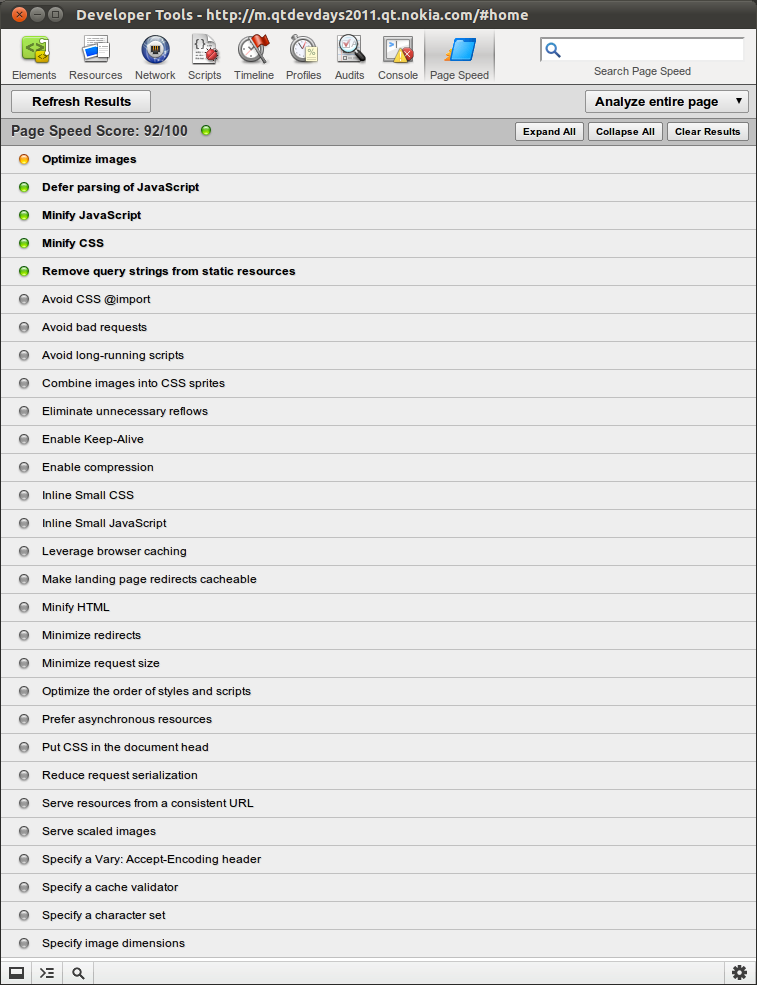
\includegraphics[width=\textwidth]{images/devdays-pagespeed.png}
    \caption{Page Speed results for the conference application.}
    \label{figure:devdays-pagespeed.png}
  \end{center}
\end{figure}

We were very happy with the Page Speed score of 92 out of 100. A lot
of the performance rules analyzed by Page Speed are similar to the
guidelines listed in Section~\ref{section:performance-guidelines}, but
there are also additional rules.

The only real problem in the score was the 'Optimize Images' rule. We
had not optimized the images used in the application, but instead used
the images provided by the designers. Going further, we could have
saved a lot or bandwidth by optimizing the images with tools such as
Pngcrush\footnote{\url{http://pmt.sourceforge.net/pngcrush/}}.

Of the other notes in the results, 'Defer parsing of JavaScript' could
have been avoided by adding a 'defer' attribute to all the script tags
in the document. The reason for this rule is that scripts block page
rendering as defined in
Section~\ref{section:performance-guidelines}. However, since we
followed the guideline 'Put Scripts at the Bottom', this rendering
issue is avoided. The only script in the document head was Modernizr,
which must be included before the page is parsed because it creates
the essential HTML5 tag support for older browsers and must do so
before the tags are parsed.

The 'Minify JavaScript' note was probably due to the Handlebars
templating library not being minified. All the JavaScript libraries
were included in their minified form, but Handlebars library was only
available unminified. We also did not want to minify it ourselves to
avoid breaking any functionality. All other JavaScript files were
minified and concatenated to avoid extra HTTP requests.

The 'Minify CSS' note was not seen as important since CSS compression
does not yield big improvements and because the CSS files were already
Gzipped delivered. The 'Remove query strings from static resources'
note means that query parameters like '?123' should be removed from
the end of the \abbr{URLs} because they might not be cached in some
proxies. We did not change this because the query strings in the
static assets were an essential part of our caching strategy.
